\documentclass[11pt]{amsart}
\usepackage[margin=1.15in]{geometry}
\usepackage{amsmath,amssymb,amsthm,mathtools}
\usepackage{graphicx}
\usepackage[dvipsnames]{xcolor}
\usepackage{booktabs}
\usepackage[colorlinks=true,linkcolor=blue!50!black,citecolor=blue!50!black,urlcolor=blue!50!black]{hyperref}
\usepackage{enumitem}

\newtheorem{theorem}{Theorem}[section]
\newtheorem{proposition}[theorem]{Proposition}
\newtheorem{lemma}[theorem]{Lemma}
\newtheorem{corollary}[theorem]{Corollary}
\newtheorem{conjecture}[theorem]{Conjecture}
\theoremstyle{definition}
\newtheorem{definition}[theorem]{Definition}
\newtheorem{assumption}[theorem]{Assumption}
\newtheorem{example}[theorem]{Example}
\theoremstyle{remark}
\newtheorem{remark}[theorem]{Remark}

\newcommand{\R}{\mathbb{R}}
\newcommand{\N}{\mathbb{N}}
\newcommand{\Pm}{\Pi_m}
\newcommand{\fp}[2]{\bigl[#1,#2\bigr]}          % Fischer pairing at the origin
\newcommand{\fpz}[3]{\bigl[#1,#2\bigr]_{#3}}     % shifted pairing
\newcommand{\todo}[1]{\textcolor{red}{[\textbf{TODO:} #1]}}
\DeclareMathOperator*{\argmin}{arg\,min}
\setlength{\emergencystretch}{2em}

\title[Hermite--Birkhoff interpolation by singular-weight MLS]{Generalized Hermite--Birkhoff
interpolation of arbitrary order in any dimension via singular-weight moving least squares}
\author{David Figueiras Garcia}
\date{Draft of \today}

\begin{document}

\begin{abstract}
Singular-weight interpolating moving least squares (SWIMLS) reproduces function values at
scattered nodes. We study the method when each node carries an arbitrary finite set of linear
differential data $q(D)f(x_i)$. We prove that the interpolant is $C^\infty$, give an exact
representation of the error in every datum, and deduce that a datum is reproduced exactly if
(i) every derivative of its symbol $q$ lies in the span of the symbols prescribed at that node
and (ii) $\Delta^{\alpha/2}q=0$, where $\alpha$ is the (even) order of the weight singularity.
Condition (ii) cannot be dropped. Whether condition (i) is needed depends on how the fit to the
other nodes moves near $x_i$: we identify configurations in which it is not needed, and give the
error explicitly when (i) fails only at first order. For classical Hermite data of order $k$, all data are reproduced
if and only if $\alpha>k$ (the necessity under a mild condition on the other nodes), which
proves a sharpened form of a conjecture of Komargodski and Levin. We also give exact
counterexamples, in one and two dimensions, to their claim that derivatives prescribed at
points without function values are interpolated, and a completion procedure that makes such
data exact. A stable evaluator and experiments in one to three dimensions confirm the theory, and in a
two-dimensional study the root-mean-square error decays at rates close to $h^{m+1}$ for local
degree $m$.
\end{abstract}

\maketitle

% ===========================================================================
\section{Introduction}\label{sec:intro}
Moving least squares (MLS) builds an approximant point by point: at each evaluation point $x$
one fits a polynomial to the data by weighted least squares, with weights that decay away from
$x$, and evaluates the fit at $x$. The method goes back to McLain~\cite{McLain1974,McLain1976}
and Lancaster and \v{S}alkauskas~\cite{LancasterSalkauskas1981}; its approximation theory is
due to Levin~\cite{Levin1998} and Wendland~\cite{Wendland2005}, see also~\cite{Fasshauer2007}.
When the weights are singular at the nodes, $w_i(x)=|x-x_i|^{-\alpha}$, the approximant
interpolates the data~\cite{LancasterSalkauskas1981}; with constant local polynomials it is
Shepard's method~\cite{Shepard1968}. Interpolating MLS needs no mesh and no global linear
system, and it is local, smooth and exact on polynomials of the local degree; MLS is also
optimal in the sense of Backus and Gilbert~\cite{BosSalkauskas1989}, and nearly interpolating
weights are used to impose boundary conditions in meshless methods~\cite{MostBucher2005}.

In many applications the data include derivatives: slopes and curvatures in curve and surface
design, gradients in derivative-enhanced surrogate models, fluxes and normal derivatives in
meshless discretisations of differential equations. Kernel methods handle such
Hermite--Birkhoff data by building the derivatives into the kernel
matrix~\cite{Wu1992,NarcowichWard1994}, at the price of a global system. In meshless methods, derivative data
have been built into MLS fits~\cite{AtluriChoKim1999}, and generalized MLS approximates
derivatives and other functionals from values~\cite{MirzaeiSchabackDehghan2012}. For
interpolating MLS, Komargodski and Levin~\cite{KomargodskiLevin2006} proposed using the same
singular weights for value and derivative data at a node. They proved that this interpolates
values and first derivatives in one dimension, and reported that for data up to second
derivatives $\alpha=2$ is not enough while $\alpha=4$ works. They conjectured that $\alpha=2k$
suffices for derivatives up to order $k$, and stated that the method also interpolates
directional derivatives prescribed at points that carry no function value.

Polynomial Hermite--Birkhoff interpolation in several variables is notoriously delicate: whether
a data pattern is poised depends on the pattern and on the geometry of the
nodes~\cite{LorentzJetterRiemenschneider1983,GascaSauer2000,Lorentz2000}; the natural class
of local data is that of D-invariant spaces~\cite{deBoorRon1990,SauerXu1995}, which
characterise ideal interpolation~\cite{deBoor2005,Shekhtman2010}.
Interpolating MLS avoids the global poisedness question, since it only asks that the data be unisolvent on the local
polynomial space. It replaces it by a local question: which data are reproduced? This paper
answers that question.

We call the method SWIMLS (singular-weight interpolating moving least squares) and analyse it
for arbitrary finite sets of linear differential data $q(D)f(x_i)$ at each node, in any
dimension. The analysis rests on two elementary tools, the Fischer pairing of a symbol with a
polynomial and a structure theorem for the local fit near a node, and it leads to an exact
formula for the error in each datum.

\paragraph{Contributions.}
\begin{enumerate}[label=(\arabic*)]
  \item A structure theorem for SWIMLS near a node (Theorem~\ref{thm:structure}): the
        interpolant is $C^\infty$, and an exact representation of the error in any differential
        datum (Theorem~\ref{thm:error}).
  \item A sufficient condition for exact reproduction of a datum $q(D)f(x_i)$: closure of the
        symbol under differentiation and $\Delta^{\alpha/2}q=0$ (Corollary~\ref{cor:exact}).
        The second condition cannot be dropped: it is necessary at leading order
        (Proposition~\ref{prop:necessity}).
  \item The role of the first condition: it is not needed when the minimiser of the
        ``frozen'' problem at the other nodes does not move near $x_i$ (Theorem~\ref{thm:frozen}),
        e.g.\ for a single other node or locally proportional weights; when it fails only at
        first order, the error is given explicitly by Proposition~\ref{prop:firstorder}.
  \item For classical Hermite data of order $k$: all data are reproduced when $\alpha>k$, and
        this is sharp (Corollaries~\ref{cor:hermite} and~\ref{cor:sharp}); when $\alpha\le k$
        the error is the linear functional $q\mapsto\fpz{\Delta^{\alpha/2}q}{\tau}{x_i}$ of the
        datum. This proves, for $k\ge3$ in a sharper form, the conjecture
        of~\cite[\S3]{KomargodskiLevin2006} that $\alpha=2k$ suffices.
  \item Exact counterexamples in one and two dimensions to the extension claimed
        in~\cite[\S3]{KomargodskiLevin2006} (Propositions~\ref{prop:kl}
        and~\ref{prop:kl2}), and a completion procedure that makes data with gaps exact
        (Proposition~\ref{prop:completion}).
  \item A numerically stable evaluation of SWIMLS, including the closed-form limit at the
        nodes, and numerical experiments in one, two and three dimensions.
\end{enumerate}

\paragraph{Outline.} Section~\ref{sec:example} shows the method and both failure mechanisms on
a one-dimensional example. Section~\ref{sec:setting} fixes notation, Section~\ref{sec:main}
contains the theory, and Section~\ref{sec:birkhoff} treats derivatives at points without values.
Sections~\ref{sec:evaluation} and~\ref{sec:numerics} describe the evaluator and the experiments,
and Section~\ref{sec:conclusions} lists open problems.

% ===========================================================================
\section{A one-dimensional example}\label{sec:example}
Take the nodes $x_i=i$, $i=0,1,2,3$, prescribe values $f_i$ and slopes $f'_i$, and fix the
exponent $\alpha=2$. At every point $x$ that is not a node, let $p_x$ be the quadratic
polynomial that minimises
\begin{equation}\label{eq:J1d}
  J_x(p)=\sum_{i=0}^{3}\frac{\bigl(p(x_i)-f_i\bigr)^2+\bigl(p'(x_i)-f'_i\bigr)^2}{(x-x_i)^2},
\end{equation}
and set $u(x):=p_x(x)$. The minimiser is linear in the data, so
$u=\sum_i\bigl(f_i\varphi_i+f'_i\psi_i\bigr)$ with shape functions $\varphi_i,\psi_i$; two of
them are shown in Figure~\ref{fig:1d}(a). They have the cardinal property of Hermite
interpolation: $\varphi_i(x_j)=\delta_{ij}$, $\varphi_i'(x_j)=0$, $\psi_i(x_j)=0$ and
$\psi_i'(x_j)=\delta_{ij}$. Nothing in~\eqref{eq:J1d} uses the ordering of the nodes or a mesh,
and the same definition works with any number of nodes in any dimension.

Why are the slopes reproduced? Near the node $x_1=1$, multiply~\eqref{eq:J1d} by $(x-1)^2$. The
first term becomes $(p(1)-f_1)^2+(p'(1)-f'_1)^2$ and the others are multiplied by the small
factor $t=(x-1)^2$. Write the quadratic as $p=p^*+r+c\,(y-1)^2$, where $p^*$ is the line with
value $f_1$ and slope $f'_1$ at $1$ and $r$ is a linear polynomial: the node data see $r$ but
not $c$. Balancing the two parts of the functional gives $r=O(t)$, while $c$ is determined by
the other nodes. Section~\ref{sec:main} makes this precise:
\[
  p_x(y)=p^*(y)+\nu(x)\,(y-1)^2+(x-1)^2\,\sigma(x)(y),
\]
with smooth coefficients $\nu$ and $\sigma$. At $y=x$ both correction terms vanish to second
order at $x=1$, so $u(1)=f_1$ and $u'(1)=f'_1$.

The same picture explains what can go wrong. If we also prescribe second derivatives and use
local cubics, the correction $(x-1)^2\sigma(x)(x)$ contributes $2\sigma(1)(1)$ to $u''(1)$,
and the datum $f''(1)$ is missed (Figure~\ref{fig:1d}(b): $u''(1)=1.05$ against
$f''(1)=-3.04$). With $\alpha=4$ the correction is $(x-1)^4\sigma(x)(x)$, which does not
affect the second derivative, and $f''(1)$ is reproduced. This is the rule ``$\alpha$ larger
than the order of the data'' of Corollary~\ref{cor:hermite}.

The other failure concerns gaps in the data. Prescribe values at $0$ and $2$ and slopes at $1$
and $3$ (Figure~\ref{fig:1d}(c)). At $x_1=1$ the only datum, the slope, does not see constants. The
component $\nu_0(x)$ of $p_x$ along the constants is then chosen by the other nodes, it varies with $x$, and its
derivative $\nu_0'(1)$ adds to $u'(1)$. The prescribed slope $0.306$ comes out as
$0.235$. Adding an estimate of the missing values $f(1)$ and $f(3)$ to the data, by any
method, restores exactness (Proposition~\ref{prop:completion}); the slopes are then reproduced
to the accuracy of finite differences.

\begin{figure}[t]
  \centering
  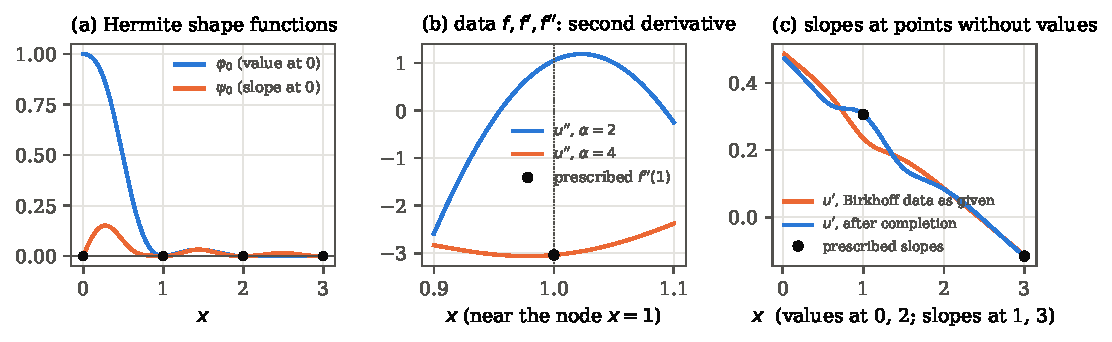
\includegraphics[width=\textwidth]{../figures/fig1_one_dimensional_example.pdf}
  \caption{The one-dimensional example. (a) Shape functions for the value and the slope at
  $x=0$ (nodes $0,1,2,3$, $m=2$, $\alpha=2$). (b) Data $f,f',f''$ at the nodes: $u''$ near the
  node $x=1$ for $\alpha=2$ and $\alpha=4$; only $\alpha=4$ reproduces $f''(1)$
  (Corollary~\ref{cor:hermite}). (c) Values at $0,2$ and slopes at $1,3$, $m=2$: the slopes are not
  reproduced (compare Proposition~\ref{prop:kl}) until the data are completed
  (Proposition~\ref{prop:completion}).}
  \label{fig:1d}
\end{figure}

% ===========================================================================
\section{Setting and notation}\label{sec:setting}

\subsection{Polynomials, symbols and the Fischer pairing}
For $d\ge1$ and $m\ge0$ let $\Pm=\Pi_m(\R^d)$ be the real polynomials of total degree at most
$m$. Multi-indices are $\beta\in\N_0^d$, with $|\beta|=\sum_j\beta_j$, $\beta!=\prod_j\beta_j!$,
$D^\beta=\partial^{|\beta|}/\partial x_1^{\beta_1}\cdots\partial x_d^{\beta_d}$. A polynomial
$q(\xi)=\sum_\beta q_\beta\xi^\beta$, called a \emph{symbol}, defines the differential operator
$q(D)=\sum_\beta q_\beta D^\beta$. We write $\partial^\gamma q$ for derivatives of a symbol with
respect to $\xi$, and $\Delta q=\sum_j\partial_j^2q$.

For a symbol $q$, a smooth function $g$ and a point $z$ we set
\begin{equation}\label{eq:pairing}
  \fpz{q}{g}{z} := \bigl(q(D)g\bigr)(z), \qquad \fp{q}{g}:=\fpz{q}{g}{0}.
\end{equation}
For polynomials $q,p$, $\fp{q}{p}=\sum_\beta\beta!\,q_\beta p_\beta$ is the \emph{Fischer inner
product}~\cite{Fischer1918,Shapiro1989}; it is positive definite on $\Pm$. Four elementary facts will be used.

\begin{lemma}[Fischer adjointness]\label{lem:fischer}
For symbols $q$ and polynomials $p$, $\fp{q}{z_jp}=\fp{\partial_jq}{p}$. Consequently
$\fp{q}{|z|^{2\ell}p}=\fp{\Delta^\ell q}{p}$ for every $\ell\in\N_0$, where
$|z|^2=\sum_jz_j^2$.
\end{lemma}

\begin{proof}
With $e_j$ the $j$-th unit multi-index,
$\fp{q}{z_jp}=\sum_\kappa\kappa!\,q_\kappa p_{\kappa-e_j}
=\sum_\lambda(\lambda+e_j)!\,q_{\lambda+e_j}p_\lambda
=\sum_\lambda\lambda!\,(\lambda_j+1)q_{\lambda+e_j}p_\lambda=\fp{\partial_jq}{p}$.
Multiplication by $|z|^2=\sum_jz_j\cdot z_j$ is therefore adjoint to $\sum_j\partial_j^2=\Delta$,
and the second statement follows by induction.
\end{proof}

\begin{lemma}[Taylor expansion of operators]\label{lem:taylor}
Let $A=(A_1,\dots,A_d)$ and $B=(B_1,\dots,B_d)$ be commuting operators. For every symbol $q$,
$q(A+B)=\sum_{\gamma}\frac{1}{\gamma!}A^\gamma(\partial^\gamma q)(B)$ (a finite sum).
\end{lemma}

\begin{proof}
This is Taylor's formula $q(a+b)=\sum_\gamma\frac{a^\gamma}{\gamma!}(\partial^\gamma q)(b)$ for
the polynomial $q$, an identity in the commutative polynomial ring in $a,b$.
\end{proof}

\begin{lemma}\label{lem:harmonic-monomial}
Let $\ell\in\N_0$ and $\beta\in\N_0^d$. Then $\Delta^\ell\xi^\beta=0$ if and only if
$\sum_j\lfloor\beta_j/2\rfloor<\ell$.
\end{lemma}

\begin{proof}
By the multinomial formula,
$\Delta^\ell\xi^\beta=\sum_{|\kappa|=\ell}\frac{\ell!}{\kappa!}\,\partial^{2\kappa}\xi^\beta$,
and $\partial^{2\kappa}\xi^\beta=\frac{\beta!}{(\beta-2\kappa)!}\xi^{\beta-2\kappa}$ if
$2\kappa\le\beta$ and $0$ otherwise. Distinct $\kappa$ give distinct monomials and all
coefficients are positive, so $\Delta^\ell\xi^\beta\ne0$ if and only if some $\kappa$ with
$|\kappa|=\ell$ satisfies $2\kappa\le\beta$, i.e.\ $\sum_j\lfloor\beta_j/2\rfloor\ge\ell$.
\end{proof}

\begin{lemma}\label{lem:normpower}
Let $\alpha\in2\N$. Then
$\sum_{|\gamma|=\alpha}\frac{1}{\gamma!}\bigl(D^\gamma|x|^\alpha\bigr)(0)\,\partial^\gamma=\Delta^{\alpha/2}$
as operators on symbols.
\end{lemma}

\begin{proof}
$|x|^\alpha=\sum_{|\kappa|=\alpha/2}\frac{(\alpha/2)!}{\kappa!}x^{2\kappa}$, and
$(D^\gamma x^{2\kappa})(0)=(2\kappa)!$ if $\gamma=2\kappa$ and $0$ otherwise. Hence the left side
equals $\sum_{|\kappa|=\alpha/2}\frac{(\alpha/2)!}{\kappa!}\partial^{2\kappa}
=\bigl(\sum_j\partial_j^2\bigr)^{\alpha/2}$.
\end{proof}

\subsection{Data}
Let $\Omega\subset\R^d$ be open and $X=\{x_1,\dots,x_K\}\subset\Omega$ distinct nodes. Node
$x_i$ carries symbols $q_{i,1},\dots,q_{i,n_i}$ of degree at most $m$ and values
$y_{i,1},\dots,y_{i,n_i}\in\R$, i.e.\ the interpolation conditions
\begin{equation}\label{eq:data}
  \lambda_{i,s}(f):=\fpz{q_{i,s}}{f}{x_i}=\bigl(q_{i,s}(D)f\bigr)(x_i)=y_{i,s},
  \qquad s=1,\dots,n_i,\ i=1,\dots,K.
\end{equation}
We write $Q_i=\operatorname{span}\{q_{i,1},\dots,q_{i,n_i}\}$ for the space of symbols at
$x_i$. Every $q=\sum_sc_sq_{i,s}\in Q_i$ has a prescribed value
$y_q:=\sum_sc_sy_{i,s}$; we say that the datum $q$ is \emph{reproduced} by a function $u$ if
$\fpz{q}{u}{x_i}=y_q$. Classical Hermite data of order $k$ correspond to
$Q_i=\operatorname{span}\{\xi^\beta:|\beta|\le k\}$; any other choice will be called
Hermite--Birkhoff data. A space of symbols is \emph{D-invariant} if it is closed under
differentiation.

\begin{assumption}\label{ass:main}
\begin{enumerate}[label=(A\arabic*)]
  \item\label{A1} $\alpha\in2\N$ is even, and $w_i(x)=\rho_i(x)\,|x-x_i|^{-\alpha}$ with
        $\rho_i\in C^\infty(\Omega)$, $\rho_i>0$.
  \item\label{A2} For every $i$ the symbols $q_{i,1},\dots,q_{i,n_i}$ are linearly
        independent.
  \item\label{A3} (Unisolvency) If $p\in\Pm$ and $\lambda_{i,s}(p)=0$ for all $i,s$, then
        $p=0$.
\end{enumerate}
\end{assumption}

Since $\fpz{\cdot}{\cdot}{x_i}$ is non-degenerate on $\Pm$ (it is the Fischer pairing after
translation) and $\deg q_{i,s}\le m$, \ref{A2} is equivalent to the linear independence of the
functionals $\lambda_{i,1},\dots,\lambda_{i,n_i}$ on $\Pm$.

\begin{definition}[SWIMLS]\label{def:swimls}
For $x\in\Omega\setminus X$ let
\begin{equation}\label{eq:functional}
  J_x(p)=\sum_{i=1}^Kw_i(x)\sum_{s=1}^{n_i}\bigl(\lambda_{i,s}(p)-y_{i,s}\bigr)^2,
  \qquad p_x:=\argmin_{p\in\Pm}J_x(p),
\end{equation}
and define the interpolant $u(x):=p_x(x)$.
\end{definition}

By \ref{A1} and \ref{A3}, $J_x$ is a strictly convex quadratic on $\Pm$ for every
$x\notin X$, so $p_x$ is unique; it depends smoothly on $x\in\Omega\setminus X$ because the
coefficients of $J_x$ do and its Hessian is positive definite. Hence $u\in
C^\infty(\Omega\setminus X)$. The behaviour at the nodes is the subject of the next section.

\begin{remark}
Positive smooth factors for the individual functionals of a node can be included: the first
block of the Jacobian in the proof of Theorem~\ref{thm:structure} becomes $2L^*W(x)L$, still
invertible, and nothing else changes. If some functionals at $x_i$ are \emph{not} given the
singular factor, they must be moved from $Q_i$ to the regular part $B_x$ of the proof, and
$Q_i,N_i$ refer to the singular ones only.
\end{remark}

% ===========================================================================
\section{Main results}\label{sec:main}

Throughout this section we fix a node $x_i$ and write
\[
  N_i=\{p\in\Pm:\lambda_{i,s}(p)=0,\ s=1,\dots,n_i\}=\{p\in\Pm:\fpz{q}{p}{x_i}=0\ \forall q\in Q_i\}
\]
for the polynomials that the data at $x_i$ do not see.

\subsection{Structure near a node}

\begin{theorem}[Structure near a node]\label{thm:structure}
Let Assumption~\ref{ass:main} hold, fix an inner product on $\Pm$ and let $R=N_i^\perp$. There
are an open neighbourhood $U\subset\Omega$ of $x_i$ with $U\cap X=\{x_i\}$, a polynomial
$p_i^*\in R$ with $\lambda_{i,s}(p_i^*)=y_{i,s}$ for all $s$, and $C^\infty$ maps
$\nu:U\to N_i$ and $\sigma:U\to R$ such that
\begin{equation}\label{eq:structure}
  p_x=p_i^*+\nu(x)+|x-x_i|^{\alpha}\,\sigma(x)\qquad\text{for all }x\in U\setminus\{x_i\}.
\end{equation}
More precisely, $\nu(x)=n(x,|x-x_i|^\alpha)$ and $\sigma(x)=s(x,|x-x_i|^\alpha)$ for $C^\infty$
maps $n,s$ defined near $(x_i,0)$, and $Z(x):=n(x,0)$ is the \emph{frozen minimiser}
\begin{equation}\label{eq:frozen}
  Z(x)=\argmin_{n\in N_i}\ B_x(p_i^*+n),\qquad
  B_x(p):=\sum_{j\ne i}\frac{w_j(x)}{\rho_i(x)}\sum_{s=1}^{n_j}\bigl(\lambda_{j,s}(p)-y_{j,s}\bigr)^2 .
\end{equation}
Applying this at every node, $u$ extends to a function in $C^\infty(\Omega)$, with node value
$u(x_i)=\bigl(p_i^*+Z(x_i)\bigr)(x_i)$.
\end{theorem}

\begin{proof}
Write $\Lambda_i:\Pm\to\R^{n_i}$, $p\mapsto(\lambda_{i,s}(p))_s$, and $\Lambda_j$ likewise. By
\ref{A2} $\Lambda_i$ is surjective with kernel $N_i$, so $L:=\Lambda_i|_R:R\to\R^{n_i}$ is
bijective; put $p_i^*:=L^{-1}y_i\in R$. Every $p\in\Pm$ is uniquely $p=p_i^*+r+n$ with $r\in
R$, $n\in N_i$, and then $\Lambda_ip-y_i=Lr$.

Let $U$ be an open neighbourhood of $x_i$ containing no other node. For $x\in U\setminus\{x_i\}$
divide $J_x$ by $w_i(x)>0$:
\[
  \frac{J_x(p)}{w_i(x)}=|Lr|^2+t(x)\,B_x(p),\qquad t(x):=|x-x_i|^{\alpha},
\]
with $B_x$ as in~\eqref{eq:frozen}. Since $\alpha$ is even,
$t(x)=\bigl(\sum_k(x_k-x_{i,k})^2\bigr)^{\alpha/2}$ is a polynomial in $x$; and $x\mapsto B_x$
is a $C^\infty$ family of convex quadratics on $U$, because $\rho_i>0$ and the $w_j$, $j\ne i$,
are smooth on $U$. A polynomial $p=p_i^*+r+n$ minimises $J_x$ if and only if the gradient
vanishes (the problem is convex), that is
\[
  2L^*Lr+t(x)\nabla_RB_x(p)=0,\qquad t(x)\nabla_NB_x(p)=0,
\]
where $\nabla_R,\nabla_N$ denote the components of the gradient in $R$ and $N_i$ and $L^*$ is
the adjoint of $L$. Since $t(x)>0$ for $x\ne x_i$ we may substitute $r=t(x)\,s$ and divide by
$t(x)$, obtaining $F(x,t(x);s,n)=0$ for the map $F:U\times\R\times R\times N_i\to R\times N_i$,
\[
  F(x,t;s,n):=\Bigl(2L^*Ls+\nabla_RB_x(p_i^*+ts+n),\ \nabla_NB_x(p_i^*+ts+n)\Bigr),
\]
which is $C^\infty$ in all variables, including $t$ near $0$.

\emph{The point $(x_i,0)$.} Here $F=0$ reads $\nabla_NB_{x_i}(p_i^*+n)=0$ and
$s=-(2L^*L)^{-1}\nabla_RB_{x_i}(p_i^*+n)$. The restriction of $B_x$ to the affine space
$p_i^*+N_i$ is strictly convex for every $x\in U$: its Hessian is
$2\sum_{j\ne i}\frac{w_j(x)}{\rho_i(x)}\Lambda_j^*\Lambda_j$ restricted to $N_i$, with
$w_j(x)>0$ since $x\ne x_j$; and if $n\in N_i$ satisfies $\Lambda_jn=0$ for all $j\ne i$ then
all data functionals vanish on $n$, so $n=0$ by \ref{A3}. Hence there is exactly one solution
$(s_0,n_0)$, and $n_0=Z(x_i)$; more generally, for every $x\in U$ the equation
$F(x,0;s,n)=0$ has the unique solution $n=Z(x)$, $s=-(2L^*L)^{-1}\nabla_RB_x(p_i^*+Z(x))$.

\emph{Implicit function theorem.} At $(x_i,0;s_0,n_0)$ the derivative of $F$ with respect to
$(s,n)$ is block triangular,
\[
  \frac{\partial F}{\partial(s,n)}=
  \begin{pmatrix} 2L^*L & \bigl(\nabla^2B_{x_i}\bigr)_{RN}\\[2pt] 0 & \bigl(\nabla^2B_{x_i}\bigr)_{NN}\end{pmatrix},
\]
because every derivative with respect to $s$ of a $B$-term carries the factor $t=0$. Both
diagonal blocks are invertible ($L$ is injective; the second block is the Hessian above).
By the implicit function theorem there are a neighbourhood $U'\times(-\tau_0,\tau_0)$ of
$(x_i,0)$ and a $C^\infty$ map $(x,t)\mapsto(s(x,t),n(x,t))$ with $F(x,t;s(x,t),n(x,t))=0$;
by the uniqueness just shown, $n(x,0)=Z(x)$. Shrinking $U$ to $U'\cap\{t(x)<\tau_0\}$, for
$x\in U\setminus\{x_i\}$ the polynomial $p_i^*+t(x)s(x,t(x))+n(x,t(x))$ satisfies the gradient
equations of the strictly convex function $J_x$, hence it equals $p_x$ (only uniqueness of the
critical point of $J_x$ is used). Setting $\nu(x):=n(x,t(x))\in N_i$ and
$\sigma(x):=s(x,t(x))\in R$ gives~\eqref{eq:structure}; both maps are $C^\infty$ because $t$ is
a polynomial. Finally $u(x)=p_x(x)$ is, by~\eqref{eq:structure}, the restriction to
$U\setminus\{x_i\}$ of the $C^\infty$ function $x\mapsto(p_i^*+\nu(x)+t(x)\sigma(x))(x)$, whose
value at $x_i$ is $(p_i^*+Z(x_i))(x_i)$.
\end{proof}

\begin{remark}\label{rem:odd}
The decomposition~\eqref{eq:structure} is canonical up to the choice of the complement $R$ of
$N_i$; the node value $u(x_i)$ and all errors below do not depend on it. Evenness of $\alpha$
is used twice: to make $t(x)=|x-x_i|^\alpha$ smooth at $x_i$ (Theorem~\ref{thm:structure}) and
to make it a polynomial, so that Lemmas~\ref{lem:fischer} and~\ref{lem:normpower} apply
(Theorems~\ref{thm:error} and~\ref{thm:frozen}). If the $\rho_i$ are real analytic, the
analytic implicit function theorem shows that $u$ is real analytic. For odd $\alpha$ the function
$t$ is not smooth at $x_i$, our arguments do not apply, and we do not consider this case.
\end{remark}

\subsection{An exact error representation}

\begin{theorem}[Error representation]\label{thm:error}
With the notation of Theorem~\ref{thm:structure}, let $\tau(z):=\sigma(z)(z)$ for $z\in U$
(a $C^\infty$ scalar function). For every symbol $q$,
\begin{equation}\label{eq:error}
  \fpz{q}{u}{x_i}
  =\fpz{q}{p_i^*}{x_i}
  +\sum_{\gamma}\frac{1}{\gamma!}\,D^\gamma\Bigl[x\mapsto\fpz{\partial^\gamma q}{\nu(x)}{x_i}\Bigr](x_i)
  +\fpz{\Delta^{\alpha/2}q}{\tau}{x_i}.
\end{equation}
The $\gamma=0$ term of the middle sum is $\fpz{q}{\nu(x_i)}{x_i}$.
\end{theorem}

\begin{proof}
On $U\times\R^d$ consider the $C^\infty$ function
$\Phi(x,y)=p_i^*(y)+\nu(x)(y)+t(x)\,\sigma(x)(y)=:\Phi_1+\Phi_2+\Phi_3$, which is a
polynomial in $y$ and satisfies $u(z)=\Phi(z,z)$ for all $z\in U$, including $z=x_i$ by the
definition of the extension. By the chain rule along the diagonal,
$D_z^\beta[\Phi(z,z)]=\bigl[(D_x+D_y)^\beta\Phi\bigr](z,z)$, hence
$\fpz{q}{u}{x_i}=\bigl[q(D_x+D_y)\Phi\bigr](x_i,x_i)$. We treat the three parts.

$\Phi_1$ does not depend on $x$, so it contributes $(q(D)p_i^*)(x_i)=\fpz{q}{p_i^*}{x_i}$.

For $\Phi_2$, Lemma~\ref{lem:taylor} with $A=D_x$, $B=D_y$ gives
$q(D_x+D_y)\Phi_2=\sum_\gamma\frac{1}{\gamma!}D_x^\gamma\,(\partial^\gamma q)(D_y)\Phi_2$.
Setting $y=x_i$ commutes with $D_x$, and $\bigl((\partial^\gamma q)(D_y)\Phi_2\bigr)(x,x_i)
=\fpz{\partial^\gamma q}{\nu(x)}{x_i}$; setting $x=x_i$ gives the middle term
of~\eqref{eq:error}.

For $\Phi_3$ we use the diagonal again: its contribution is
$\fpz{q}{t\,\tau}{x_i}=\bigl(q(D)[\,|z-x_i|^\alpha\tau(z)]\bigr)(x_i)$. Translate $x_i$ to $0$
and let $T\tau$ be the Taylor polynomial of $\tau$ at $0$ of degree $\deg q$. Since
$|z|^\alpha(\tau-T\tau)$ vanishes at $0$ to order larger than $\deg q$, it is annihilated by
$q(D)$ at $0$, and by Lemma~\ref{lem:fischer}
\[
  \fp{q}{|z|^\alpha\tau}=\fp{q}{|z|^\alpha T\tau}=\fp{\Delta^{\alpha/2}q}{T\tau}
  =\fp{\Delta^{\alpha/2}q}{\tau},
\]
the last equality because $\deg\Delta^{\alpha/2}q\le\deg q-\alpha\le\deg T\tau$.
\end{proof}

\subsection{Exact reproduction}

\begin{corollary}[Sufficient condition]\label{cor:exact}
Let Assumption~\ref{ass:main} hold and let $q\in Q_i$. If
\begin{enumerate}[label=(\roman*)]
  \item\label{c1} $\partial^\gamma q\in Q_i$ for every multi-index $\gamma$, and
  \item\label{c2} $\Delta^{\alpha/2}q=0$,
\end{enumerate}
then the datum $q$ is reproduced: $\fpz{q}{u}{x_i}=y_q$. If $Q_i$ is D-invariant, the error is
the linear functional
\begin{equation}\label{eq:dinv-error}
  \fpz{q}{u}{x_i}-y_q=\fpz{\Delta^{\alpha/2}q}{\tau}{x_i},\qquad q\in Q_i .
\end{equation}
\end{corollary}

\begin{proof}
In~\eqref{eq:error}, $\fpz{q}{p_i^*}{x_i}=\sum_sc_s\lambda_{i,s}(p_i^*)=y_q$. By~\ref{c1},
every $\partial^\gamma q$ (including $\gamma=0$) lies in $Q_i$, and $\nu(x)\in N_i$, so
$\fpz{\partial^\gamma q}{\nu(x)}{x_i}=0$ for all $x\in U$: the middle term vanishes. This
proves~\eqref{eq:dinv-error} when $Q_i$ is D-invariant, and the last term vanishes
by~\ref{c2}.
\end{proof}

Condition~\ref{c1} concerns the datum and the data at its own node only; it holds for every
datum when $Q_i$ is D-invariant, the classical setting of multivariate Hermite
interpolation~\cite{SauerXu1995,deBoor2005}. Condition~\ref{c2} holds whenever $\deg q<\alpha$,
but also, for instance, for every harmonic symbol when $\alpha=2$. By~\eqref{eq:dinv-error} the
reproduced data at a D-invariant node form the subspace $\{q\in Q_i:\Delta^{\alpha/2}q=0\}$ plus
the kernel of the functional $\fpz{\cdot}{\tau}{x_i}$ on $\Delta^{\alpha/2}Q_i$; for instance, at
$\alpha=2$ the errors in $\partial_x^2f$ and $\partial_y^2f$ coincide, $\partial_x^2-\partial_y^2$
is reproduced, and the error in $\partial_x^3f$ is three times that in $\partial_x\partial_y^2f$.

\begin{corollary}[Hermite data]\label{cor:hermite}
Let $x_i$ carry classical Hermite data of order $k\le m$, i.e.\
$Q_i=\operatorname{span}\{\xi^\beta:|\beta|\le k\}$. Then every $q\in Q_i$ with
$\Delta^{\alpha/2}q=0$ is reproduced. In particular:
\begin{enumerate}[label=(\alph*)]
  \item the derivative datum $D^\beta f(x_i)$ is reproduced whenever
        $\sum_j\lfloor\beta_j/2\rfloor<\alpha/2$;
  \item all data at $x_i$ are reproduced if $\alpha>k$, i.e.\ for $\alpha=k+1$ when $k$ is odd
        and $\alpha=k+2$ when $k$ is even;
  \item for $\alpha=2$ the monomial data covered by~(a) are exactly the multilinear ones
        ($\beta_j\le1$ for all $j$, e.g.\ $\partial_x\partial_y$,
        $\partial_x\partial_y\partial_z$), whatever their order.
\end{enumerate}
\end{corollary}

\begin{proof}
$Q_i$ is D-invariant, so Corollary~\ref{cor:exact} applies; (a) and (c) are
Lemma~\ref{lem:harmonic-monomial} with $\ell=\alpha/2$, and (b) follows from
$\deg q\le k<\alpha$.
\end{proof}

Corollary~\ref{cor:hermite}(b) proves the conjecture of~\cite[\S3]{KomargodskiLevin2006} that
$\alpha=2k$ suffices for data up to order $k$ (they also observed that $\alpha=2$ fails and
$\alpha=4$ works for $k=2$). Their conjecture refers to ``an appropriate definition of the
inner product'', which they do not specify; we read it as the same singular weight for all data
at a node, as in their one-dimensional construction. For $k\ge3$ Corollary~\ref{cor:hermite}(b) is a strict improvement, e.g.\ $\alpha=4$ suffices
for $k=3$. The next result shows that condition~\ref{c2} cannot be dropped, and with it that
(b) is sharp (Corollary~\ref{cor:sharp}).

\begin{proposition}[Necessity of \ref{c2}, leading order]\label{prop:necessity}
In addition to Assumption~\ref{ass:main}, assume that the data at the nodes other than $x_i$
are unisolvent on $\Pm$ by themselves. Let $q\in Q_i$ satisfy~\ref{c1}, with $\deg q=\alpha$
and $\Delta^{\alpha/2}q\ne0$. Then, for every choice of the data at $x_i$, the datum $q$ is
reproduced only if the data at the other nodes lie in a fixed affine hyperplane.
\end{proposition}

\begin{proof}
By~\ref{c1} the middle term of~\eqref{eq:error} vanishes, and $\Delta^{\alpha/2}q=c$ is a
non-zero constant, so the error is $c\,\tau(x_i)=c\,\sigma(x_i)(x_i)=c\,s_0(x_i)$ with $s_0$
from the proof of Theorem~\ref{thm:structure}. The error is an affine function of the data at
the other nodes (with $y_i$ fixed); it vanishes for the data $y_j=\Lambda_jp_i^*$, so it
suffices to exhibit data for which it does not.

Since $\deg q=\alpha\ge2$, some derivative $\partial^\gamma q$ with $|\gamma|=\alpha$ is a
non-zero constant, so $1\in Q_i$ by~\ref{c1}: point evaluation $\ell(p)=p(x_i)$ is a datum at
$x_i$. It vanishes on $N_i$ and is non-zero on $\Pm$, hence non-zero on $R$.

Choose $y_j=\Lambda_j(p_i^*+v)$, $j\ne i$, for some $v\in\Pm$. Then
$B_{x_i}(p)=\langle K(p-p_i^*-v),p-p_i^*-v\rangle$ with
$K=\sum_{j\ne i}\frac{w_j(x_i)}{\rho_i(x_i)}\Lambda_j^*\Lambda_j$, which is positive definite on
$\Pm$ by the additional assumption. The minimiser $n_0$ over $N_i$ is characterised by
$K(n_0-v)\perp N_i$, i.e.\ $K(n_0-v)\in R$, so $\nabla_RB_{x_i}(p_i^*+n_0)=2K(n_0-v)$ and
$s_0=(L^*L)^{-1}Kw$ with $w=v-n_0$. As $v$ ranges over $\Pm$, $w$ ranges over the
$K$-orthogonal complement $W=\{w:Kw\in R\}$ of $N_i$, so $Kw$ ranges over all of $R$ and
$s_0$ over all of $R$. Choosing $v$ with $\ell(s_0)\ne0$ completes the proof.
\end{proof}

\begin{corollary}[Sharpness]\label{cor:sharp}
Under the hypotheses of Proposition~\ref{prop:necessity} on the other nodes, let $x_i$ carry
classical Hermite data of order $k\le m$. If $\alpha\le k$, the datum $\partial_1^\alpha f(x_i)$
is not reproduced for data at the other nodes outside an affine hyperplane. Hence $\alpha>k$ is
the exact condition for all Hermite data of order $k$ to be reproduced for all data values.
\end{corollary}

\begin{proof}
$q=\xi_1^\alpha\in Q_i$ satisfies~\ref{c1} by D-invariance, $\deg q=\alpha$ and
$\Delta^{\alpha/2}\xi_1^\alpha=\alpha!\ne0$.
\end{proof}

\subsection{The role of condition~\ref{c1}}

When~\ref{c1} fails, the middle term of~\eqref{eq:error} involves derivatives of $\nu$, which
are governed by how the weights of the \emph{other} nodes vary near $x_i$. Two situations can be
described completely.

\begin{theorem}[Frozen minimiser]\label{thm:frozen}
Let Assumption~\ref{ass:main} hold and suppose that the frozen minimiser $Z$
of~\eqref{eq:frozen} is constant near $x_i$. Then every $q\in Q_i$ with $\deg q\le\alpha$
satisfies
\begin{equation}\label{eq:frozen-error}
  \fpz{q}{u}{x_i}-y_q=\fpz{\Delta^{\alpha/2}q}{\partial_tn(x_i,0)+\tau}{x_i},
\end{equation}
where $\Delta^{\alpha/2}q$ is a constant. In particular every $q\in Q_i$ with $\deg q<\alpha$, or
with $\deg q=\alpha$ and $\Delta^{\alpha/2}q=0$, is reproduced, whether or not~\ref{c1} holds.
\end{theorem}

\begin{proof}
By Theorem~\ref{thm:structure}, $\nu(x)=n(x,t(x))$ with $n(x,0)=Z(x)$ constant, so
$\nu(x)=Z(x_i)+t(x)\,g(x)$ with $g(x)=\int_0^1\partial_tn(x,\theta t(x))\,d\theta$ smooth and
$g(x_i)=\partial_tn(x_i,0)$. Since $t$ vanishes at $x_i$ to order $\alpha$,
$D^\gamma[t\,g](x_i)=0$ for $|\gamma|<\alpha$ and $D^\gamma[t\,g](x_i)=(D^\gamma t)(x_i)\,g(x_i)$
for $|\gamma|=\alpha$. In the middle term of~\eqref{eq:error}: the $\gamma=0$ term is
$\fpz{q}{\nu(x_i)}{x_i}=0$ because $q\in Q_i$ and $\nu(x_i)\in N_i$; the terms with
$0<|\gamma|<\alpha$ vanish because the constant $Z(x_i)$ is killed by $D^\gamma$ and $t\,g$ has
vanishing derivatives of these orders; the terms with $|\gamma|>\alpha$ vanish because
$\partial^\gamma q=0$; and the terms with $|\gamma|=\alpha$, in which $\partial^\gamma q$ is a
constant, add up by Lemma~\ref{lem:normpower} to
\[
  \sum_{|\gamma|=\alpha}\frac{1}{\gamma!}(D^\gamma t)(x_i)\,\fpz{\partial^\gamma q}{g(x_i)}{x_i}
  =\fpz{\Delta^{\alpha/2}q}{\partial_tn(x_i,0)}{x_i}.
\]
Together with $\fpz{q}{p_i^*}{x_i}=y_q$ and the last term of~\eqref{eq:error} this
gives~\eqref{eq:frozen-error}.
\end{proof}

\begin{corollary}\label{cor:frozen-cases}
The frozen minimiser is constant near $x_i$, and hence Theorem~\ref{thm:frozen} applies, in each
of the following cases:
\begin{enumerate}[label=(\alph*)]
  \item \emph{single scale:} $w_j(x)/\rho_i(x)=c(x)\kappa_j$ near $x_i$ for all $j\ne i$, with a
        positive function $c$ and constants $\kappa_j>0$; this includes the case of a single
        other node ($K=2$) and weights whose germs at $x_i$ are proportional;
  \item \emph{interpolatory restriction:} the functionals $\lambda_{j,s}$, $j\ne i$, that do not
        vanish identically on $N_i$ restrict to a basis of the dual of $N_i$ (so that the frozen
        problem can fit them exactly whatever the weights).
\end{enumerate}
\end{corollary}

\begin{proof}
(a) $B_x=c(x)\hat B$ with $\hat B$ independent of $x$, and the minimiser of $c(x)\hat B$ over
$p_i^*+N_i$ does not depend on $c(x)>0$. (b) The frozen objective is a positively weighted sum
of squared residuals of functionals that are either constant on $p_i^*+N_i$ or, by assumption,
can be made zero simultaneously by exactly one $n\in N_i$, which is then the minimiser for
every choice of positive weights.
\end{proof}

\begin{example}
These cases are not exotic: for two nodes, gradient data at $x_i$ without a function value are
reproduced for $\alpha\ge2$; in one dimension with $m=1$, the data $f'(0)$, $f(1)$, $f'(5/2)$
are all reproduced (case (b): only $f(1)$ sees the constants, which form $N_i$ at the slope
nodes). A third node in the first case, or a further value datum in the second, destroys the
structure, and the data are then no longer reproduced (Section~\ref{sec:numerics}).
\end{example}

In general the frozen minimiser moves, and a failure of~\ref{c1} at first order produces an
explicit error.

\begin{proposition}[First-order error]\label{prop:firstorder}
Let Assumption~\ref{ass:main} hold and let $q\in Q_i$ with $\deg q<\alpha$, such that
$\partial^\gamma q\in Q_i$ for all $|\gamma|\ge2$. Then
\begin{equation}\label{eq:firstorder}
  \fpz{q}{u}{x_i}-y_q=\sum_{j=1}^d\fpz{\partial_jq}{\partial_{x_j}Z(x_i)}{x_i},\qquad
  \partial_{x_j}Z(x_i)=-H^{-1}\,\partial_{x_j}\bigl[\nabla_NB_x\bigr](p_i^*+Z(x_i))\Big|_{x=x_i},
\end{equation}
where $H$ is the Hessian of $B_{x_i}$ restricted to $N_i$.
\end{proposition}

\begin{proof}
In~\eqref{eq:error} the last term vanishes because $\deg q<\alpha$, and the middle terms with
$\gamma=0$ or $|\gamma|\ge2$ vanish as in Corollary~\ref{cor:exact}. For $|\gamma|=1$,
$D_j\fpz{\partial_jq}{\nu(x)}{x_i}=\fpz{\partial_jq}{\partial_{x_j}\nu(x_i)}{x_i}$ and
$\partial_{x_j}\nu(x_i)=\partial_{x_j}n(x_i,0)+\partial_tn(x_i,0)\,\partial_jt(x_i)
=\partial_{x_j}Z(x_i)$ since $\alpha\ge2$. Differentiating $\nabla_NB_x(p_i^*+Z(x))=0$ gives the
formula for $\partial_{x_j}Z$.
\end{proof}

The right-hand side of~\eqref{eq:firstorder} is an explicit linear functional of the data; for
pure power weights ($\rho\equiv1$) it is a rational function of the node positions. It
vanishes in the cases of Corollary~\ref{cor:frozen-cases} and for symmetric configurations (e.g.\
$\partial_{x_1}w_j(x_i)=0$ for all $j$), but it is non-zero in the explicit examples of
Section~\ref{sec:birkhoff}, and therefore, by analyticity, for node positions in an open dense
set for those data patterns.

\begin{conjecture}\label{conj:char}
Let $\rho\equiv1$, let $Q_i$ be D-invariant and the other nodes unisolvent by themselves. If
$\Delta^{\alpha/2}q\ne0$ then, for node positions outside a proper algebraic subset, $q$ is not
reproduced for data outside a hyperplane.
\end{conjecture}

\begin{remark}
Proposition~\ref{prop:necessity} proves the conjecture for $\deg q=\alpha$. It is supported by
the experiments of Section~\ref{sec:numerics} (e.g.\ $\partial_x^2\partial_yf$ at $\alpha=2$ fails
even for $K=2$). Characterising the node configurations for which a failure of~\ref{c1}
causes an error, beyond the first-order formula~\eqref{eq:firstorder}, is open.
\end{remark}

% ===========================================================================
\section{Derivative data without function values}\label{sec:birkhoff}

\subsection{Counterexamples}
Komargodski and Levin~\cite[\S3]{KomargodskiLevin2006} extend their Hermite MLS, with weights
$|x-z|^{-\alpha}$, $\alpha\in2\N$, and local spaces containing the constants and the linear
functions, to directional derivatives prescribed at points that need not carry function values,
and state that the derivative data are interpolated, the proof being ``straightforward \dots\ by
slight modifications'' of the co-located case. Condition~\ref{c1} fails for such data: the
symbol of a first derivative differentiates to the constant $1$, which is not in $Q_i$ when no
value is prescribed at the node. By Theorem~\ref{thm:frozen} this does not always cause an
error, but it can, and does in the following examples, computed in exact rational arithmetic
(scripts in \texttt{code/proofs}). In the second example the gradient is given as two
directional derivatives at the same point, as~\cite[\S3]{KomargodskiLevin2006} allow for
gradient data.

\begin{proposition}\label{prop:kl}
Let $d=1$, $m=1$ (local polynomials $a+by$), $\alpha=2$, $\rho_i\equiv1$, and prescribe
$f(0)=f(2)=0$ and $f'(1)=f'(3)=1$. Then
\[
  u(x)=\frac{x\,(x-1)(x-2)\,(x^2-4x+5)}{2x^4-14x^3+37x^2-42x+19},
\]
which satisfies $u(0)=u(2)=0$ but $u'(1)=-1$ and $u'(3)=31/25$.
\end{proposition}

\begin{proof}
With $w_z(x)=(x-z)^{-2}$ the normal equations of~\eqref{eq:functional} for $(a,b)$ are
\[
  \begin{pmatrix} w_0+w_2 & 2w_2\\ 2w_2 & 4w_2+w_1+w_3\end{pmatrix}
  \begin{pmatrix} a\\ b\end{pmatrix}=\begin{pmatrix} 0\\ w_1+w_3\end{pmatrix},
\]
whose solution gives $u=a+bx$ as stated; the denominator has no real zeros. The remaining
values follow by direct computation.
\end{proof}

\begin{proposition}\label{prop:kl2}
Let $d=2$, $m=1$, $\alpha=2$, $\rho_i\equiv1$, and prescribe $f=0$ at $(0,0)$, $(2,0)$, $(0,2)$
and $\nabla f(1,1)=(1,1)$. With $s=x_1+x_2$, $r=x_1^2+x_2^2$ and $p=x_1x_2$,
\[
  u=\frac{15sr^2-68r^2-64pr+128sr+16ps-128r-96p+48s}{35r^2-120sr+240r+208p-240s+144},
\]
which vanishes at the three value points, while $\nabla u(1,1)=(5/9,5/9)$.
\end{proposition}

\begin{proof}
Exact computation as in Proposition~\ref{prop:kl}, with three unknowns (script in
\texttt{code/proofs}). The denominator tends to $+\infty$ as $|x|\to\infty$, and its
minimum, attained on the diagonal near $(0.898,0.898)$, is $11.21\ldots>0$.
\end{proof}

The failure persists for $\alpha=4$ and for $m=2$ (Section~\ref{sec:numerics}).

\subsection{Completion}
Given data at $x_i$ with symbol space $Q_i$, let $\overline{Q}_i$ be the smallest D-invariant
space containing $Q_i$; it has the same maximal degree as $Q_i$, since differentiation lowers
degrees. Choose a basis $\tilde q_{i,1},\dots,\tilde q_{i,r}$ of a complement of $Q_i$ in
$\overline{Q}_i$.

\begin{proposition}[Completion]\label{prop:completion}
Augment the data at $x_i$ by the functionals $\tilde q_{i,l}(D)f(x_i)$ with arbitrary values
$\tilde y_{i,l}$. If Assumption~\ref{ass:main} holds for the original data, it holds for the
augmented data, and every original datum $q\in Q_i$ with $\Delta^{\alpha/2}q=0$ (in particular
every datum of order less than $\alpha$) is reproduced by the augmented interpolant, whatever
the values $\tilde y_{i,l}$.
\end{proposition}

\begin{proof}
The augmented symbols at $x_i$ form a basis of $\overline{Q}_i$, so~\ref{A2} holds;
\ref{A3} is preserved by adding data. The prescribed value $y_q$ of an original datum is
unchanged, because its representation in the augmented basis is unique. Every
$q\in Q_i\subset\overline{Q}_i$ satisfies~\ref{c1} with respect to the D-invariant space
$\overline{Q}_i$, and Corollary~\ref{cor:exact} applies.
\end{proof}

The values $\tilde y_{i,l}$ influence the accuracy, not the exactness. In the experiments they
are estimated by a smooth (non-singular) moving least-squares fit of the given data.

% ===========================================================================
\section{Numerical evaluation}\label{sec:evaluation}
The usual implementation of interpolating MLS replaces $|x-x_i|^{-\alpha}$ by
$(|x-x_i|^\alpha+\varepsilon)^{-1}$ and solves the normal equations. This gives up exactness at
the nodes and, near a node, squares the condition number of the weighted system, which grows
like $|x-x_i|^{-\alpha/2}$.
Our evaluator avoids both problems. All of it is in the accompanying code.

\paragraph{Basis and weights.} At the evaluation point $x$ we use the monomials
$((y-x)/h)^\beta$, $|\beta|\le m$, with a length scale $h$, so that $u(x)$ is the first
coefficient. The weights are either pure powers $|x-x_i|^{-\alpha}$ or
$w_i(x)=|x-x_i|^{-\alpha}e^{-|x-x_i|^2/\delta^2}$, which also satisfy~\ref{A1}; they are computed as logarithms and normalised by their maximum, and
nodes whose normalised weight is below a cutoff are dropped. The cutoff is measured relative to
the strongest node \emph{other than} the nearest one; measured relative to the nearest node,
it would drop all other nodes close to a node and destroy the information that fixes $\nu$.
Rows of derivative data of order $r$ are multiplied by $\ell^{r}$ for a length $\ell$; by the
remark after Definition~\ref{def:swimls} this does not affect the results of
Section~\ref{sec:main}.

\paragraph{Least squares.} The weighted system $W^{1/2}A\,a\approx W^{1/2}b$ is solved by an
SVD-based least-squares solver rather than through the normal equations. Close to a node $x_i$
the rows of $x_i$ dominate the others by a factor $s^{-1}$ with $s\sim|x-x_i|^{\alpha/2}$. The
light rows carry the information that fixes $\nu(x)$, and a standard solver resolves them only
to relative accuracy of order $\varepsilon_{\mathrm{mach}}/s$ (and not at all through the normal
equations once $s^2<\varepsilon_{\mathrm{mach}}$). When $s<10^{-3}$ we therefore solve an exact reformulation. Let $R$ and $L$ be
the heavy and light rows, $Q_1$ and $Q_2$ orthonormal bases of the row space and the null space
of $R$, and $c_0$ the least-squares solution of $RQ_1c=b_R$. Writing
$a=Q_1(c_0+s\,d)+Q_2z$ and dividing the objective by $s^2$ gives the problem
\[
  \min_{d,z}\ \|RQ_1d\|^2+\bigl\|LQ_1d+s^{-1}LQ_2z-s^{-1}(b_L-LQ_1c_0)\bigr\|^2,
\]
whose blocks are well scaled; it has the same minimiser and is the discrete counterpart of the
decomposition~\eqref{eq:structure}.

\paragraph{At the nodes.} At $x=x_i$, and within a tolerance of $10^{-13}$ times the size of the
node set, we use the limit of Theorem~\ref{thm:structure}: the data
at $x_i$ are imposed as equality constraints, and the remaining freedom in $N_i$ is fixed by
minimising the frozen functional~\eqref{eq:frozen}; then $u(x_i)=(p_i^*+Z(x_i))(x_i)$.

\paragraph{Accuracy.} Figure~\ref{fig:stability} compares the evaluator with a reference
computed with 120 significant digits, as the evaluation point approaches a node. Its error
stays at the level of rounding (below $5\cdot10^{-15}$) down to distance $10^{-14}$; the three smallest distances are within the node
tolerance and use the formula at the node. With $\varepsilon=10^{-10}$ the
regularised normal equations have errors up to $1.6\cdot10^{-10}$, the size of the
regularisation; with $\varepsilon=10^{-16}$ the errors reach $4\cdot10^{-12}$ and the matrix is
numerically singular at some distances.

\begin{figure}[t]
  \centering
  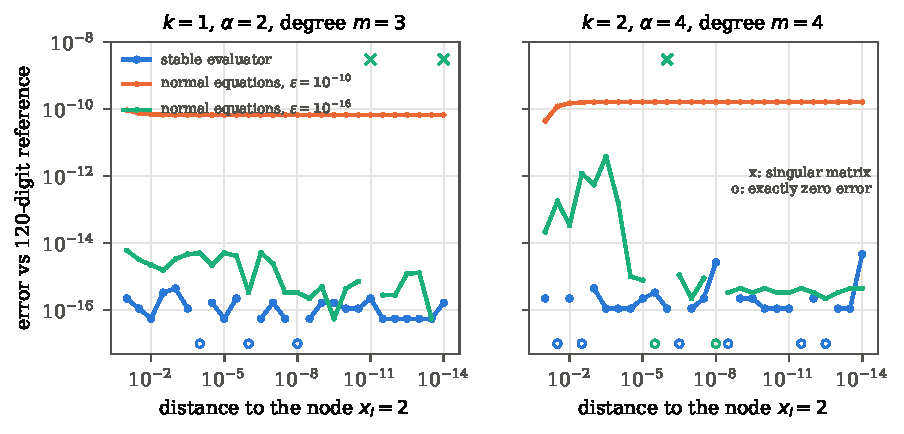
\includegraphics[width=0.9\textwidth]{../figures/e5_stability.pdf}
  \caption{Error of the evaluation near the node $x_i=2$ (nodes $1,2,3,4$ with Hermite data of
  order $k$ and random values), against a 120-digit reference. Crosses mark singular normal
  equations, open circles errors that are exactly zero.}
  \label{fig:stability}
\end{figure}

\paragraph{Verifying exactness.} The experiments below decide whether a datum $q$ is reproduced
by computing $\fpz{q}{u}{x_i}$ in high-precision arithmetic (\texttt{mpmath}). The interpolant
is evaluated from the normal equations at a working precision of
$40+(2\alpha+|\beta|+5)\,|\log_{10}r|$ digits, and derivatives are taken with tensor-product
Chebyshev stencils of radius $r$ that are exact for polynomials of degree
$|\beta|+5$ in each variable and never sample the node itself. A datum is called reproduced if
$|\fpz{q}{u}{x_i}-y_q|\le10^{-12}\max(1,|y_q|)$ for both $r=10^{-6}$ and $r=10^{-4}$, and not
reproduced if the inequality fails for both. Mixed outcomes never occurred. In all reproduced
cases the error scales like the stencil error $r^{6}$ (about $10^{-30}$ and $10^{-20}$), while
in the others it is the same at both radii to the digits shown.

% ===========================================================================
\section{Numerical experiments}\label{sec:numerics}
All experiments use the evaluator and the verification procedure of
Section~\ref{sec:evaluation}; scripts, logs and data are in the accompanying repository. Unless
stated otherwise, nodes are random (in one dimension they are fixed and irregular), the weights
include the Gaussian factor of Section~\ref{sec:evaluation}, the data values are random numbers (exactness does not
depend on them being samples of a function), and every node other than the one under study
carries Hermite data, so that the generic situation of Section~\ref{sec:main} applies.

\subsection{Hermite data}
We checked every datum at one node for classical Hermite data of order $k$ in one, two and three
dimensions: $(d,k,\alpha)=(1,5,4)$, $(1,7,6)$, $(2,2,2)$, $(2,3,2)$, $(2,3,4)$, $(2,4,4)$,
$(3,2,2)$ and $(3,3,2)$, with $m=k+1$ or $k+2$; and a two-dimensional node carrying the
D-invariant space of harmonic symbols of degree at most $3$ ($1$, $\xi_1$, $\xi_2$,
$\xi_1\xi_2$, $\xi_1^2-\xi_2^2$, $\xi_1^3-3\xi_1\xi_2^2$, $3\xi_1^2\xi_2-\xi_2^3$) at $\alpha=2$. In all $92$ data,
the datum is reproduced exactly when $\Delta^{\alpha/2}q=0$ and is not reproduced otherwise,
as Corollary~\ref{cor:hermite} predicts and as Conjecture~\ref{conj:char} would predict for
pure power weights. For instance, at
$\alpha=2$ in three dimensions with $k=3$, $\partial_x\partial_y\partial_z f$ is reproduced while
$\partial_x^2 f$ has error $30$.

At a node with Hermite data of order $3$ in two dimensions and $\alpha=2$, the signed errors
satisfy the identities that follow from~\eqref{eq:dinv-error}, namely
$e(\partial_x^2)=e(\partial_y^2)=-45.904682196$, $e(\partial_x^3)=3e(\partial_x\partial_y^2)
=599.09999304$ and $e(\partial_y^3)=3e(\partial_x^2\partial_y)=-31.441788804$, to all twelve
digits computed, while $f,\partial_xf,\partial_yf,\partial_x\partial_yf$ are reproduced.

\subsection{Hermite--Birkhoff data}\label{sec:hb-num}
Next one node carries a pattern with gaps: in one dimension the orders $\{0,2\}$, $\{0,3\}$,
$\{1\}$, $\{2\}$, $\{1,2\}$, $\{0,1,3\}$ and $\{0,2,3\}$ (and two complete patterns), with
$\alpha=8$, $m=5$; in two dimensions ten patterns such as $\{f,\partial_{xx}\}$,
$\{f,\partial_x,\partial_{xy}\}$, $\{f,\Delta\}$, $\{\partial_x\}$ and a directional
derivative, with $\alpha=6$, $m=3$; four patterns at $\alpha=2$; and the two settings of
Section~\ref{sec:kl-num} ($17$ data, $m=2$, $\alpha=2$). Since $\alpha$ exceeds the order of
the data in the first two groups and in the last one, condition~\ref{c2} holds there, and only~\ref{c1} decides.
In all $83$ data the outcome agrees with conditions~\ref{c1} and~\ref{c2}: for example
$\partial_{xy}f$ is not reproduced in the pattern $\{f,\partial_x,\partial_{xy}\}$, because its
derivative $\xi_2$ is missing, and the Laplacian is not reproduced in $\{f,\Delta\}$.

\subsection{Configurations of Theorem~\ref{thm:frozen}}
Condition~\ref{c1} fails in each of the following configurations, and yet the data are
reproduced, as Theorem~\ref{thm:frozen} and Proposition~\ref{prop:firstorder} predict. Each
configuration is followed by a small perturbation that destroys the special structure, after
which the datum is no longer reproduced (two random data vectors each).

\smallskip
\begin{center}\small
\begin{tabular}{@{}llll@{}}
\toprule
configuration & datum & reason & error\\
\midrule
1D: $f'(0)$, $f(1)$, $f'(5/2)$; $m=1$, $\alpha=2$ & $f'$ at $0$, $5/2$ & Cor.~\ref{cor:frozen-cases}(b) & $<10^{-36}$\\
\quad add $f(4)$ & & & $0.21$--$2.1$\\
2D, $K=2$: $\nabla f(x_1)$; $f,\nabla f,\nabla^2f$ at $x_2$; $m=2$, $\alpha=2$ & $\partial_x,\partial_y$ & Cor.~\ref{cor:frozen-cases}(a) & $<10^{-31}$\\
\quad add a third node & & & $0.03$--$0.46$\\
2D, $K=2$: $f,\partial_{xx}f$ at $x_1$; Hermite $k=2$ at $x_2$; $\alpha=4$ & $\partial_{xx}$ & Cor.~\ref{cor:frozen-cases}(a) & $<10^{-21}$\\
\quad add a third node & & & $2.9$--$3.3$\\
2D: $\partial_xf(0)$; others on the $x_2$-axis; $m=1$, $\alpha=2$ & $\partial_x$ & Prop.~\ref{prop:firstorder} & $<10^{-29}$\\
\quad move the others by $0.05$ & & & $0.08$--$0.16$\\
\bottomrule
\end{tabular}
\end{center}
\smallskip

\noindent In the symmetric configuration the weights of the other nodes are even in $x_1$, so
$\partial_{x_1}Z(x_i)=0$ and the right-hand side of~\eqref{eq:firstorder} vanishes for
$q=\xi_1$. The experiments in the previous subsection avoid such configurations by using random
node positions.

\subsection{Derivatives at points without values}\label{sec:kl-num}
In the setting of~\cite[\S3]{KomargodskiLevin2006}: eight random points carry values and eight
other points carry gradients, the weights are $|x-x_i|^{-\alpha}$ and the local space is
$\Pi_1$ or $\Pi_2$. For all four combinations of $m\in\{1,2\}$ and $\alpha\in\{2,4\}$ the value
checked is reproduced, but none of the $24$ gradient components checked (three gradient points) is: the
errors lie between $0.06$ and $4.5$. After completion (Proposition~\ref{prop:completion}), the $6$ gradient
components checked for $m=2$, $\alpha=2$ (with a Gaussian factor in the weights) are reproduced.
Completion also repairs all $13$ non-reproduced data of the Birkhoff patterns of
Section~\ref{sec:hb-num} whose order is less than $\alpha$.

Completion does cost accuracy. With values at $n$ Halton points and gradients at $n$ others
for Franke's function ($m=3$, $\alpha=2$), the maximum error on $[0.1,0.9]^2$ for $n=1024$ is
$1.2\cdot10^{-3}$ without and $3.4\cdot10^{-3}$ with completion. In exchange, the mismatch of
the gradients drops from $4.4\cdot10^{-2}$ to the level of the finite differences used to
measure it. The added values were estimated by a simple Gaussian-weighted least-squares fit;
better estimators would reduce the penalty.

\subsection{Convergence}\label{sec:convergence}
We do not prove convergence orders, and report what a parameter study shows. The nodes are
$N=64,\dots,4096$ consecutive points of the Halton sequence (skipping the first $31$) in $[0,1]^2$, the data are values (and
gradients, and Hessians) of $f(x,y)=e^{x+y/2}\cos 2y+\sin 3xy$, the weights carry a Gaussian
factor of width $\delta=ch$ with $h=N^{-1/2}$, and errors are measured on a $33\times33$ grid in
$[0.1,0.9]^2$. We varied $c\in\{1.5,2,3,4\}$ ($c\in\{2,3,4,5\}$ for values with $m\ge4$), the data order
$k\in\{0,1,2\}$, the degree $m\in\{2,\dots,5\}$ and $\alpha\in\{2,4\}$ with $\alpha>k$, in
$44$ combinations.

\begin{itemize}
  \item \emph{Rates.} Over the last three refinements, the root-mean-square error decays like
        $h^{\,r}$ with $|r-(m+1)|\le0.53$ in every combination, i.e.\ at the rate known for MLS
        approximation with local degree $m$~\cite{Levin1998,Wendland2005}. The maximum error is
        less regular, with rates between $m-0.3$ and $m+1.6$. The rate is governed by $m$; we
        see no systematic dependence on $k$ or $\alpha$.
  \item \emph{Width.} At $N=4096$ the narrowest Gaussian tried ($c=1.5$, or $c=2$ where
        $1.5$ was not run) gives the smallest error in every case; the widest one costs a
        factor between $2.6$ and $54$ in the error. The observed rates also change with $c$, by
        up to $1.35$ for the maximum error and $0.7$ for the root-mean-square error, so the
        finest grids are not yet fully asymptotic.
  \item \emph{Hermite data.} On a fixed node set, derivative data reduce the error
        (Figure~\ref{fig:convergence}(a)): for $N=4096$ and $m=5$ from $5.0\cdot10^{-9}$ (values) to
        $1.1\cdot10^{-9}$ (values, gradients and Hessians). Per number of data, however, values
        alone were more accurate in this experiment (Figure~\ref{fig:convergence}(b)). Derivative
        data pay off when nodes are expensive and derivatives are cheap, as with adjoint
        gradients, rather than per datum.
\end{itemize}

\begin{figure}[t]
  \centering
  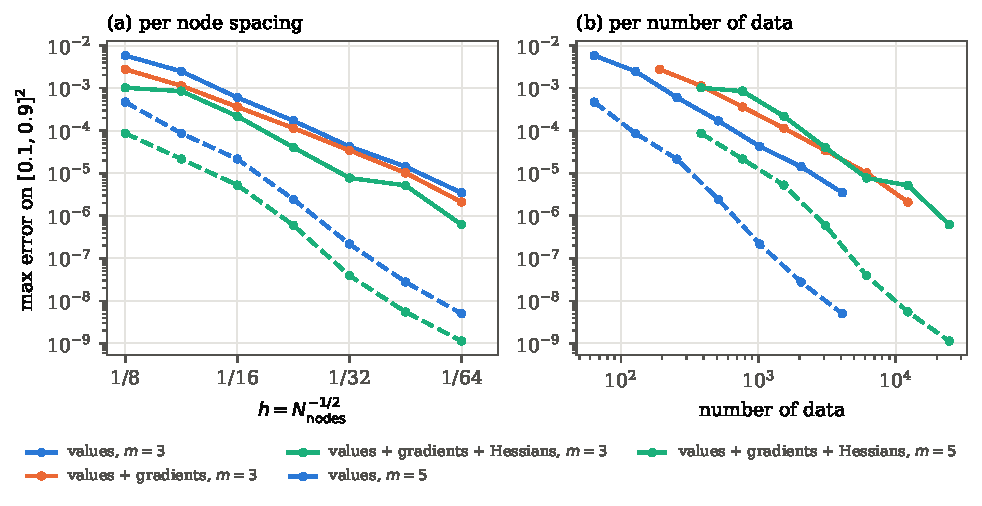
\includegraphics[width=\textwidth]{../figures/e7_convergence.pdf}
  \caption{Maximum error on $[0.1,0.9]^2$ for Halton nodes, $\delta=2h$; $\alpha=2$ except for
  Hessian data ($\alpha=4$). (a) Against the node spacing. (b) Against the total number of data.}
  \label{fig:convergence}
\end{figure}

% ===========================================================================
\section{Conclusions}\label{sec:conclusions}
Singular-weight moving least squares extends from function values to arbitrary linear
differential data with no change to its definition: one weighted least-squares problem per
evaluation point, with no mesh, no global system and no poisedness condition beyond
unisolvency of all the data on the local polynomial space. The interpolant is $C^\infty$, and
Theorem~\ref{thm:error} accounts exactly for the error in every datum. Two mechanisms can
spoil a datum: the singularity of the weight, which acts through $\Delta^{\alpha/2}$, and the
motion of the frozen minimiser, which acts only on data whose derivatives are missing at their
node. The first is removed by choosing $\alpha$ larger than the order of the data, the second by
completing the data at the node. Together they give a simple recipe for Hermite--Birkhoff
interpolation of any order in any dimension.

Several questions remain open. Conjecture~\ref{conj:char} asks whether $\Delta^{\alpha/2}q\ne0$
always causes an error in generic configurations; we proved it at leading order. Beyond the
first-order formula~\eqref{eq:firstorder}, we do not know exactly which configurations of the
other nodes make condition~\ref{c1} unnecessary. The convergence orders observed in
Section~\ref{sec:convergence} call for an error analysis in the spirit
of~\cite{Levin1998,Wendland2005} that accounts for derivative data and singular weights.
Finally, the values added by completion affect the accuracy, not the exactness, and better
ways of estimating them would reduce the accuracy penalty observed in
Section~\ref{sec:numerics}.

% ===========================================================================
\bibliographystyle{amsplain}
\begin{thebibliography}{99}

\bibitem{AtluriChoKim1999}
S.~N. Atluri, J.~Y. Cho, and H.-G. Kim, \emph{Analysis of thin beams, using the meshless local {P}etrov--{G}alerkin method, with generalized moving least squares interpolations}, Comput. Mech. \textbf{24} (1999), no.~5, 334--347, doi:10.1007/s004660050456.
% verified: https://link.springer.com/article/10.1007/s004660050456

\bibitem{BosSalkauskas1989}
L.~Bos and K.~\v{S}alkauskas, \emph{Moving least-squares are {B}ackus--{G}ilbert optimal}, J. Approx. Theory \textbf{59} (1989), no.~3, 267--275.
% verified: https://iris.univr.it/handle/11562/429372

\bibitem{deBoor2005}
C.~de Boor, \emph{Ideal interpolation}, Approximation Theory XI: Gatlinburg 2004 (C.~K. Chui, M.~Neamtu, and L.~L. Schumaker, eds.), Nashboro Press, Brentwood, TN, 2005, pp.~59--91.
% verified: https://ftp1.cs.wisc.edu/Approx/texasxi.pdf

\bibitem{deBoorRon1990}
C.~de Boor and A.~Ron, \emph{On multivariate polynomial interpolation}, Constr. Approx. \textbf{6} (1990), no.~3, 287--302, doi:10.1007/BF01890412.
% verified: https://rd.springer.com/article/10.1007/BF01890412

\bibitem{Fasshauer2007}
G.~E. Fasshauer, \emph{Meshfree Approximation Methods with {MATLAB}}, Interdisciplinary Mathematical Sciences, vol.~6, World Scientific, Singapore, 2007, doi:10.1142/6437.
% verified: https://www.worldscientific.com/worldscibooks/10.1142/6437

\bibitem{Fischer1918}
E.~Fischer, \emph{{\"U}ber die {D}ifferentiationsprozesse der {A}lgebra}, J. Reine Angew. Math. \textbf{148} (1918), 1--78, doi:10.1515/crll.1918.148.1.
% verified: https://eudml.org/doc/149470

\bibitem{GascaSauer2000}
M.~Gasca and T.~Sauer, \emph{Polynomial interpolation in several variables}, Adv. Comput. Math. \textbf{12} (2000), no.~4, 377--410, doi:10.1023/A:1018981505752.
% verified: https://www.doi.org/10.1023/A:1018981505752

\bibitem{KomargodskiLevin2006}
Z.~Komargodski and D.~Levin, \emph{Hermite type moving-least-squares approximations}, Comput. Math. Appl. \textbf{51} (2006), no.~8, 1223--1232, doi:10.1016/j.camwa.2006.04.005.
% verified against the PDF (Section 3 read in full)

\bibitem{LancasterSalkauskas1981}
P.~Lancaster and K.~\v{S}alkauskas, \emph{Surfaces generated by moving least squares methods}, Math. Comp. \textbf{37} (1981), no.~155, 141--158, doi:10.1090/S0025-5718-1981-0616367-1.
% verified: https://www.ams.org/journals/mcom/1981-37-155/S0025-5718-1981-0616367-1/

\bibitem{Levin1998}
D.~Levin, \emph{The approximation power of moving least-squares}, Math. Comp. \textbf{67} (1998), no.~224, 1517--1531, doi:10.1090/S0025-5718-98-00974-0.
% verified: https://www.doi.org/10.1090/S0025-5718-98-00974-0

\bibitem{Lorentz2000}
R.~A. Lorentz, \emph{Multivariate {H}ermite interpolation by algebraic polynomials: a survey}, J. Comput. Appl. Math. \textbf{122} (2000), no.~1--2, 167--201.
% verified: https://ftp.math.utah.edu/pub/tex/bib/idx/jcomputapplmath2000/122/1/167_201.html

\bibitem{LorentzJetterRiemenschneider1983}
G.~G. Lorentz, K.~Jetter, and S.~D. Riemenschneider, \emph{Birkhoff Interpolation}, Encyclopedia of Mathematics and its Applications, vol.~19, Addison-Wesley, Reading, MA, 1983.
% verified: https://www.cambridge.org/core/books/birkhoff-interpolation/B6518A0D062D7337A14EF193103274CD

\bibitem{McLain1974}
D.~H. McLain, \emph{Drawing contours from arbitrary data points}, Comput. J. \textbf{17} (1974), no.~4, 318--324, doi:10.1093/comjnl/17.4.318.
% verified: Franke 1982 (Math. Comp.) reference list

\bibitem{McLain1976}
D.~H. McLain, \emph{Two dimensional interpolation from random data}, Comput. J. \textbf{19} (1976), no.~2, 178--181, doi:10.1093/comjnl/19.2.178.
% verified: zbMATH 0321.65009

\bibitem{MirzaeiSchabackDehghan2012}
D.~Mirzaei, R.~Schaback, and M.~Dehghan, \emph{On generalized moving least squares and diffuse derivatives}, IMA J. Numer. Anal. \textbf{32} (2012), no.~3, 983--1000, doi:10.1093/imanum/drr030.
% verified: https://academic.oup.com/imajna/article-abstract/32/3/983/675168

\bibitem{MostBucher2005}
T.~Most and C.~Bucher, \emph{A moving least squares weighting function for the element-free {G}alerkin method which almost fulfills essential boundary conditions}, Struct. Eng. Mech. \textbf{21} (2005), no.~3, 315--332, doi:10.12989/sem.2005.21.3.315.
% verified: https://koreascience.kr/article/JAKO200521349891864.do

\bibitem{NarcowichWard1994}
F.~J. Narcowich and J.~D. Ward, \emph{Generalized {H}ermite interpolation via matrix-valued conditionally positive definite functions}, Math. Comp. \textbf{63} (1994), no.~208, 661--687, doi:10.1090/S0025-5718-1994-1254147-6.
% verified: https://www.ams.org/mcom/1994-63-208/S0025-5718-1994-1254147-6/

\bibitem{SauerXu1995}
T.~Sauer and Y.~Xu, \emph{On multivariate {H}ermite interpolation}, Adv. Comput. Math. \textbf{4} (1995), no.~1, 207--259, doi:10.1007/BF03177515.
% verified: https://link.springer.com/article/10.1007/BF03177515

\bibitem{Shapiro1989}
H.~S. Shapiro, \emph{An algebraic theorem of {E}.~{F}ischer, and the holomorphic {G}oursat problem}, Bull. London Math. Soc. \textbf{21} (1989), no.~6, 513--537, doi:10.1112/blms/21.6.513.
% verified: https://academic.oup.com/blms/article/21/6/513/344154

\bibitem{Shekhtman2010}
B.~Shekhtman, \emph{Ideal interpolation: translations to and from algebraic geometry}, Approximate Commutative Algebra, Texts and Monographs in Symbolic Computation, Springer, Vienna, 2010, doi:10.1007/978-3-211-99314-9\_6.
% verified: https://link.springer.com/chapter/10.1007/978-3-211-99314-9_6

\bibitem{Shepard1968}
D.~Shepard, \emph{A two-dimensional interpolation function for irregularly-spaced data}, Proceedings of the 1968 23rd ACM National Conference, ACM, New York, 1968, pp.~517--524, doi:10.1145/800186.810616.
% DOI not checked against the ACM page (unreachable)

\bibitem{Wendland2005}
H.~Wendland, \emph{Scattered Data Approximation}, Cambridge Monographs on Applied and Computational Mathematics, vol.~17, Cambridge University Press, Cambridge, 2005, doi:10.1017/CBO9780511617539.
% verified: https://www.cambridge.org/core/books/scattered-data-approximation/980EEC9DBC4CAA711D089187818135E3

\bibitem{Wu1992}
Z.~Wu, \emph{Hermite--{B}irkhoff interpolation of scattered data by radial basis functions}, Approx. Theory Appl. \textbf{8} (1992), no.~2, 1--10, doi:10.1007/BF02836101.
% verified: https://link.springer.com/article/10.1007/BF02836101

\end{thebibliography}

\end{document}
